\begin{frame}[t]{ALTERNATIVMETHODE}
		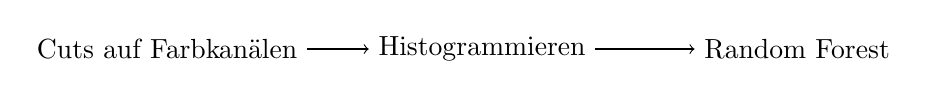
\begin{tikzpicture}[node distance=4cm]
				\node (A) {Cuts auf  Farbkanälen};
				\node (B) [right of=A, ] {Histogrammieren};
				\node (C) [right of=B] {Random Forest};
		
				\draw [->, right of=A] (A) -- (B);
				\draw [->] (B) -- (C);
		\end{tikzpicture}
  \begin{columns}
    \begin{column}{0.5\textwidth}
      \centering
      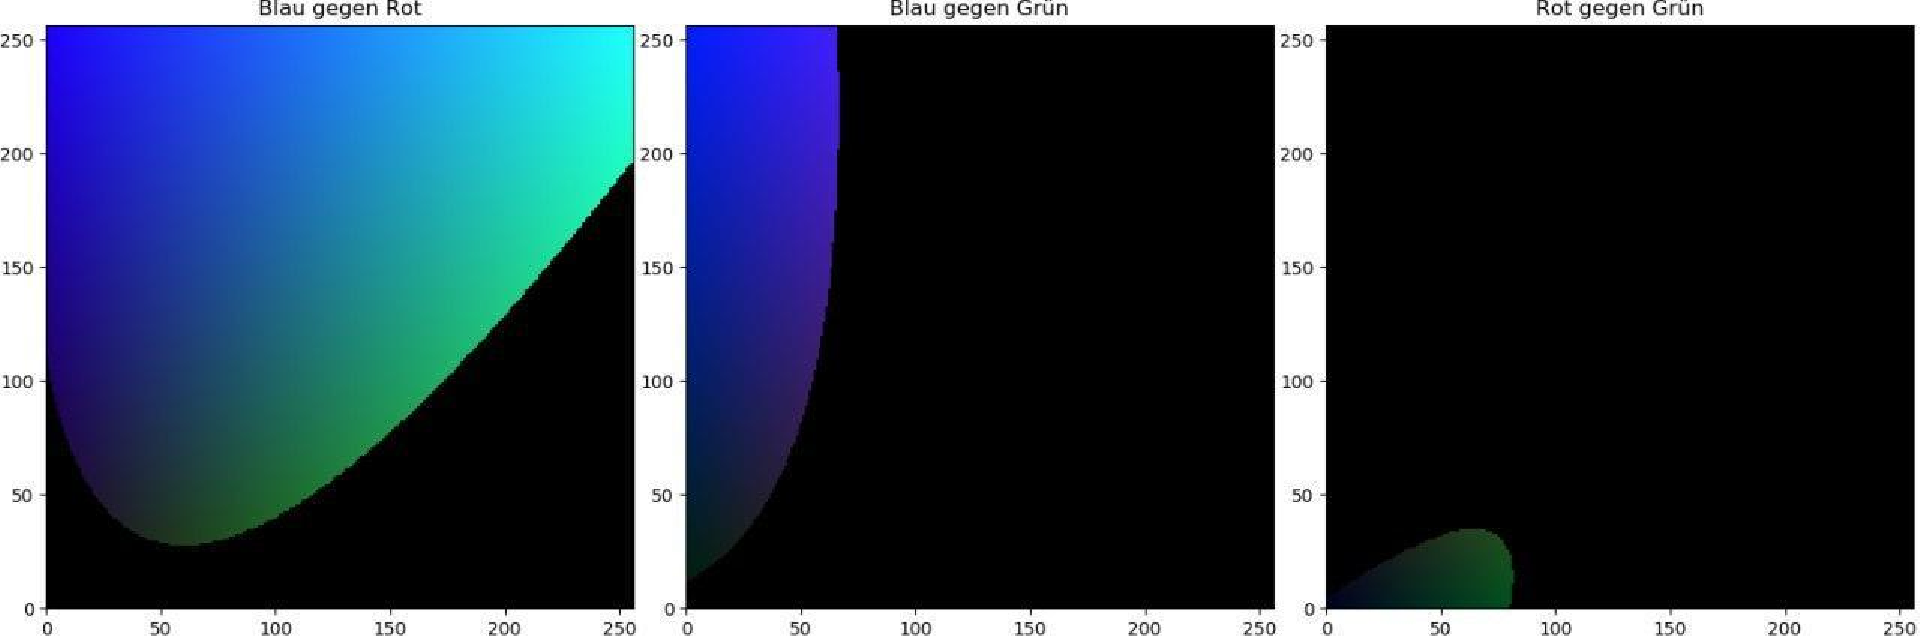
\includegraphics[width=\textwidth]{content/colorcuts1.pdf}

      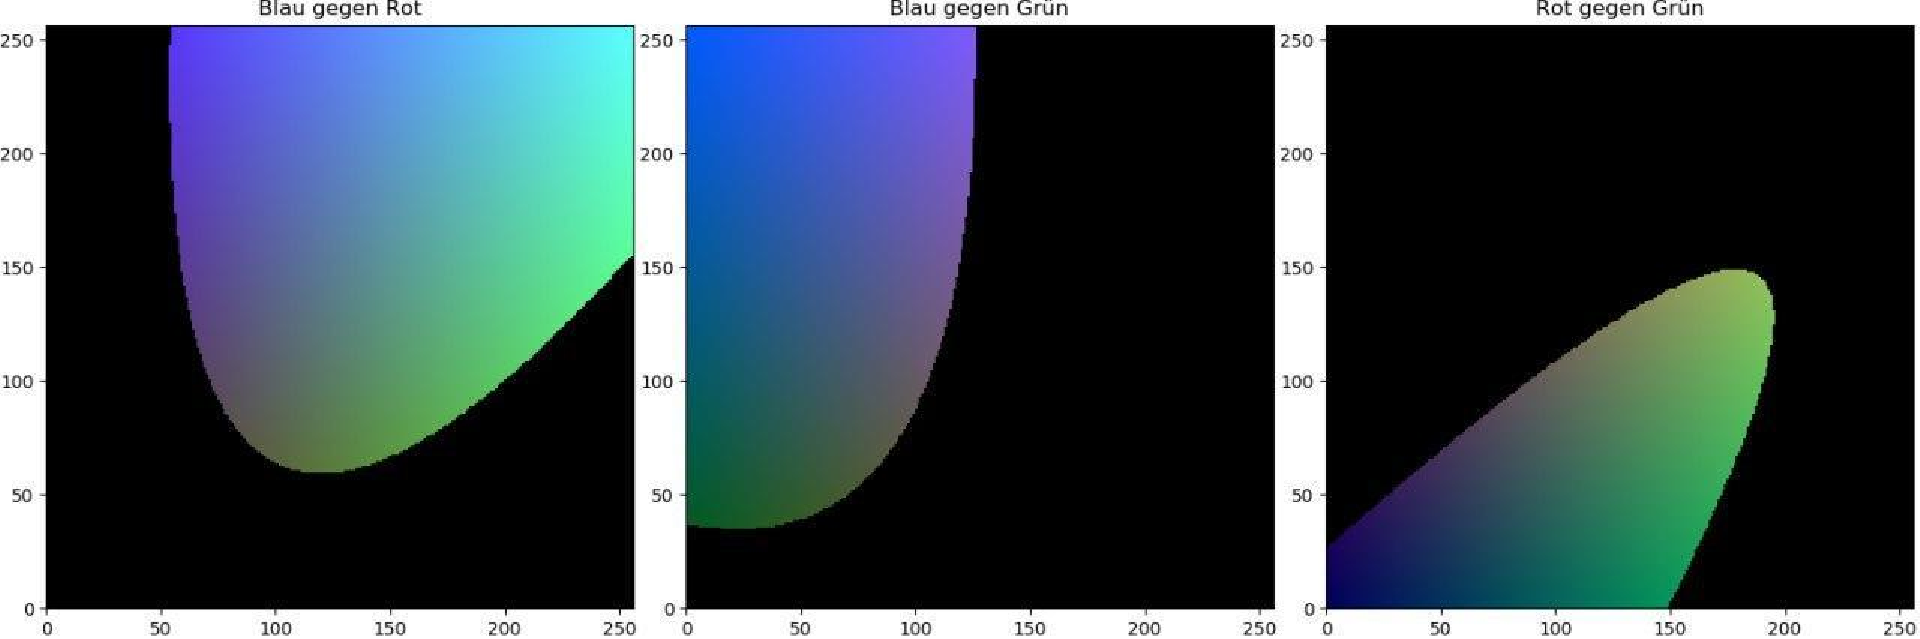
\includegraphics[width=\textwidth]{content/colorcuts2.pdf}

      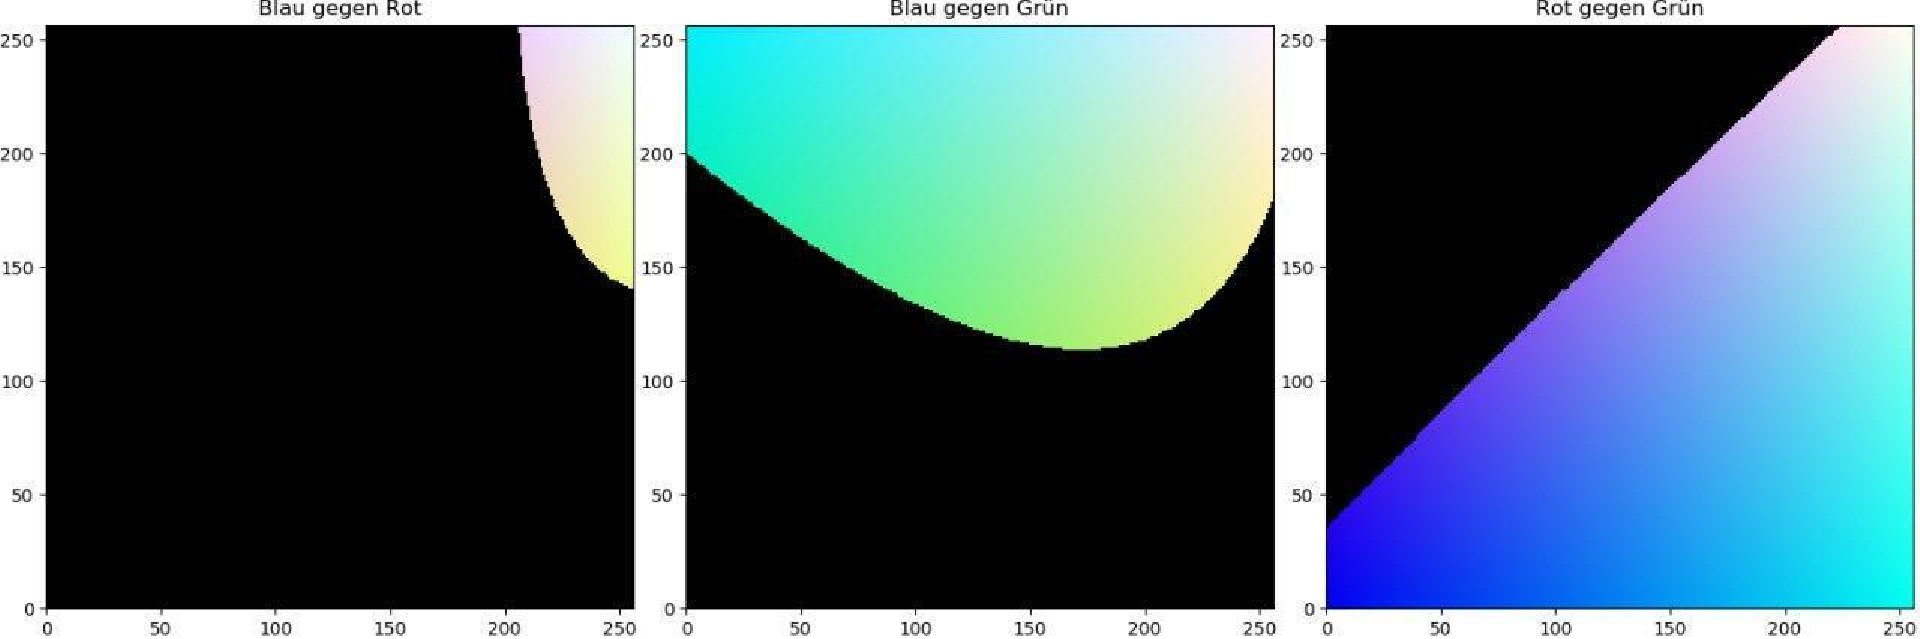
\includegraphics[width=\textwidth]{content/colorcuts3.pdf}
    \end{column}
    \begin{column}{0.5\textwidth}
      \centering
      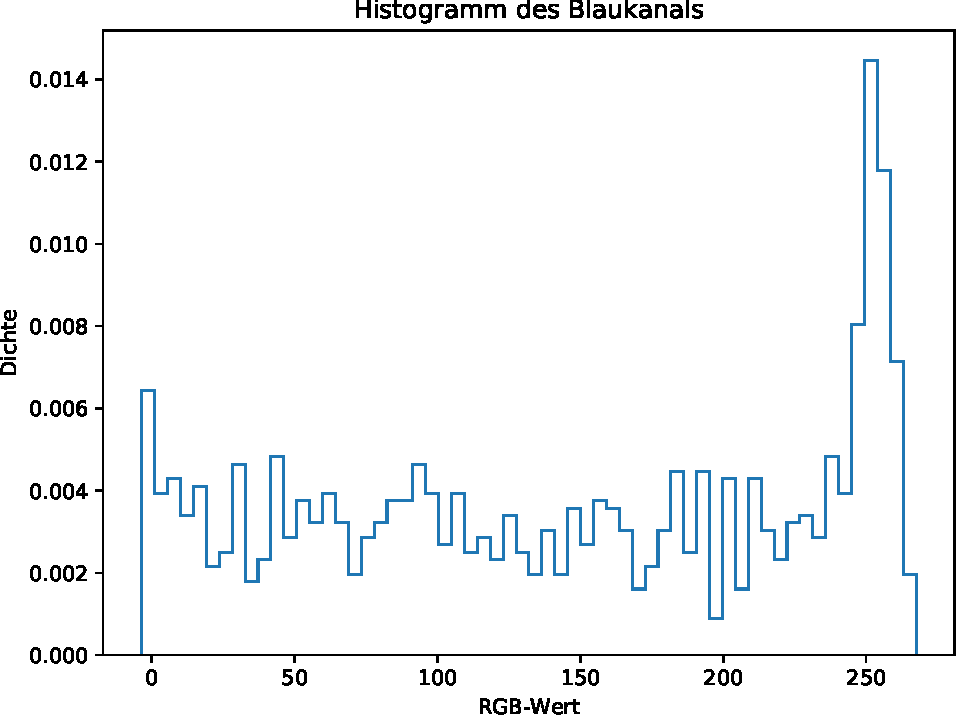
\includegraphics[width=\textwidth]{content/hist.pdf}
    \end{column}
  \end{columns}
  \centering

  $\Rightarrow$ \SI{40}{\percent} Genauigkeit
\end{frame}
